\documentclass[10pt]{beamer}

\usetheme[progressbar=frametitle]{metropolis}

\include{preamble}

\usepackage{booktabs}
\usepackage[scale=2]{ccicons}

%\usepackage{pgfplots}
%\usepgfplotslibrary{dateplot}

\usepackage{xspace}
\newcommand{\themename}{\textbf{\textsc{metropolis}}\xspace}

\title{Large-Scale Optimization Techniques}
\subtitle{and Applications to Vehicle Routing}
\date{December 1, 2016}
\author{Kamyar Khodamoradi}
\institute{Simon Fraser University \\ School of Computing Science}
\titlegraphic{\hfill\includegraphics[height=0.75cm]{logo_sfu}}

\begin{document}

\maketitle

\begin{frame}{Table of contents}
  \setbeamertemplate{section in toc}[sections numbered]
  \tableofcontents[hideallsubsections]
\end{frame}

%%%%%%%%%%%%%%%%%%%%%%%%%%%%%%%%%%%%%%%%%%%%%%%%%%%%%%%%%%%%%%%%%%%%%%%%%%%%%%%%%%%%%%%%%%%%%%%%%%%%%%%%%%%%%%%%%%%%%%%%%%%%%%%
\section{Vehicle Routing Problems}

\begin{frame}{Introduction (1)} 
    \begin{itemize}
        \item<1-> Vehicle Routing problem (VRP) is a major problem in the logistics and delivery services
        \item<2-> Skill Vehicle Routing Problem:
            \begin{itemize}
                \item<3-> Utility service company
                \item<4-> Customers request service on a daily basis
                \item<5-> The company sends service people to customers
            \end{itemize}    
    \end{itemize}
\end{frame}

\begin{frame}[t]{SVRP (1)}
    \begin{example}
        \begin{center}
            \includegraphics[width=8cm]{VRPSS01.pdf} 
        \end{center}
    \end{example}
\end{frame}

\begin{frame}[t]{SVRP (2)}
    \begin{example}
        \begin{center}
            \includegraphics[width=8cm]{VRPSS02.pdf} 
        \end{center}
    \end{example}
\end{frame}

\begin{frame}[t]{SVRP (3)}
    \begin{example}
        \begin{center}
            \includegraphics[width=8cm]{VRPSS03.pdf} 
        \end{center}
    \end{example}
\end{frame}

% \begin{frame}[t]{SVRP (4)}
%     \begin{example}
%         \begin{center}
%             \includegraphics[width=8cm]{VRPSS01.pdf} 
%         \end{center}
%     \end{example}
% \end{frame}

\begin{frame}[t]{SVRP (5)}
    \begin{itemize}
        \item<1-> We use a technique based on Linear Programming (LP) to solve SVRP
        \item<2-> \alert{Column Generation}
            \begin{itemize}
                \item<3-> Master problem: SVRP
                \item<4-> Subproblem: \textbf{Prize Collecting Traveling Salesman Problem (PCTSP)}
            \end{itemize}
        \item<5-> We need to solve PCTSP optimally
    \end{itemize}
\end{frame}

\begin{frame}[t]{Prize Collecting TSP (1)}
    \begin{itemize}
        \item<1-> Traveling Salesman Problem (TSP):
            \begin{itemize}
                \item<2-> Metric graph $G = (S, \, E)$ (on a Euclidean plane) 
                \item<3-> A special node ``depot'', $r \in S$
                \item<4-> A cost function $c:E \rightarrow \bR^+$ for every pair of nodes        
                \item<5-> Objective: Find a tour covering the depot and \alert{all} other nodes, \alert{minimizing the sum of the costs}
            \end{itemize}
    \end{itemize}
\end{frame}

\begin{frame}[t]{Prize Collecting TSP (2)}
    \begin{itemize}
        \item<1-> PCTSP:
            \begin{itemize}
                \item<2-> Metric graph $G = (S, \, E)$ (on a Euclidean plane) 
                \item<2-> A special node ``depot'', $r \in S$
                \item<2-> A cost function $c:E \rightarrow \bR^+$ for every pair of nodes
                \item<3-> A \alert{prize} function $\beta:S \rightarrow \bR^+$ for every node
                \item<4-> Objective: Find a tour covering the depot and \alert{some} other nodes, \alert{maximizing the sum of prizes minus the sum of costs}
            \end{itemize}
    \end{itemize}
\end{frame}

\begin{frame}[fragile]{An Example (1)}

\begin{itemize}
\item An instance of the Prize Collecting TSP:
\begin{figure}
	\centering
	\begin{tikzpicture}
        
        \draw (0, 0) node[circle, inner sep=1pt, fill=black, label={below:{$depot$}}] (D) {}; 
        \draw (1, 1) node[circle, inner sep=1pt, fill=black] (A) {}; 
        \draw (3, 2) node[circle, inner sep=1pt, fill=black] (B) {}; 
        \draw (-3, 3) node[circle, inner sep=1pt, fill=black] (C) {}; 
        \draw (-1, 4) node[circle, inner sep=1pt, fill=black] (E) {}; 
        \draw (0, 3) node[circle, inner sep=1pt, fill=black] (F) {}; 
        \draw (2, 3) node[circle, inner sep=1pt, fill=black] (G) {}; 
         \draw (-3, 1) node[circle, inner sep=1pt, fill=black, label={below:{$v$}}] (v) {}; 
        \draw (-2, 2) node[circle, inner sep=1pt, fill=black, label={below:{$u$}}] (u) {};         
        \node at (-2.5, 1.5) (m) {};
        \node at (-4, 1.5) (n) {$c_{uv}$};
        
        \draw [->, color = red] (m) to [bend right = 45] (n);
        \draw [fill = blue, dashed, thick] (u) to (v);

    	\node[above = 0.2cm] at (-2, 2) {$\beta_u$};
	\end{tikzpicture}
\end{figure}
\end{itemize}
\end{frame}

\begin{frame}[fragile]{An Example (2)}

\begin{itemize}
\item Solution value $ = (6 + 2 + 7 + 10 + 4) - (3.2  + 1.4 + 2.2 + 3.2 + 2.2 + 1.4) = $ \alert{15.4}
\begin{figure}
	\centering
	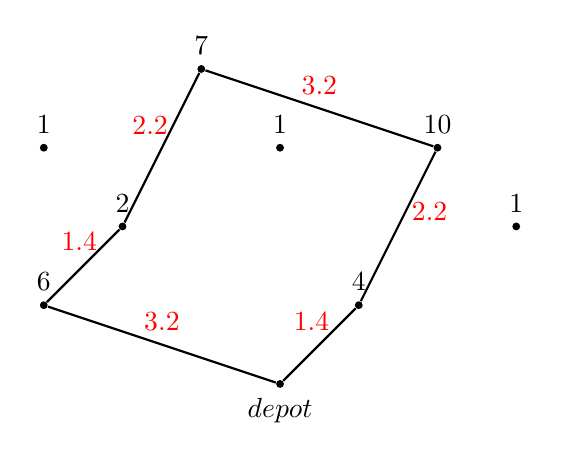
\begin{tikzpicture}
        
        \draw (0, 0) node[circle, inner sep=1pt, fill=black, label={below:{$depot$}}] (D) {}; 
        \draw (1, 1) node[circle, inner sep=1pt, fill=black, label = {above:{4}}] (A) {}; 
        \draw (3, 2) node[circle, inner sep=1pt, fill=black, label = {above:{1}}] (B) {}; 
        \draw (-3, 3) node[circle, inner sep=1pt, fill=black, label = {above:{1}}] (C) {}; 
        \draw (-1, 4) node[circle, inner sep=1pt, fill=black, label = {above:{7}}] (E) {}; 
        \draw (0, 3) node[circle, inner sep=1pt, fill=black, label = {above:{1}}] (F) {}; 
        \draw (2, 3) node[circle, inner sep=1pt, fill=black, label = {above:{10}}] (G) {}; 
         \draw (-3, 1) node[circle, inner sep=1pt, fill=black, label = {above:{$6$}}] (v) {}; 
        \draw (-2, 2) node[circle, inner sep=1pt, fill=black, label = {above:{$2$}}] (u) {};                 
        \draw [fill = blue, thick] (D) to (v) to (u) to (E) to (G) to (A) to (D);
        \node [above = 0.05cm, color = red] at (-1.5, 0.5) {3.2};
        \node [above = 0.07cm, color = red] at (-2.55, 1.5) {1.4};
        \node [above = 0.05cm, color = red] at (-1.65, 3) {2.2};
        \node [above = 0.05cm, color = red] at (0.5, 3.5) {3.2};
        \node [above = 0.05cm, color = red] at (1.9, 1.9) {2.2};
        \node [above = 0.05cm, color = red] at (0.4, 0.5) {1.4};
        
	\end{tikzpicture}
\end{figure}
\end{itemize}
\end{frame}

%%%%%%%%%%%%%%%%%%%%%%%%%%%%%%%%%%%%%%%%%%%%%%%%%%%%%%%%%%%%%%%%%%%%%%%%%%%%%%%%%%%%%%%%%%%%%%%%%%%%%%%%%%%%%%%%%%%%%%%%%%%%%%%
\section{The Branch-and-Cut Algorithm}


\begin{frame}{ILP-Based Solution}
    \begin{itemize}
        \item<1-> Our method: Branch-and-Cut
        \item<2-> Based on Integer Lienar Programming (ILP) formulation of the problem
        \item<3-> LP vs. ILP:
            \begin{itemize}
                \item<4-> LP is generally \emph{easy}
                    \begin{itemize}
                        \item<5-> Polynomial time solvable: the \textbf{Elipsoid} method
                        \item<6-> Exponential time but efficient: \textbf{Simplex} algorithm
                        \item<7-> Probably polynomial and efficient: \textbf{Karmarkar} algorithm
                    \end{itemize}
                \item<8-> ILP is \emph{hard}
                    \begin{itemize}
                        \item<9-> \emph{NP}-complete
                        \item<10-> Computationally time consuming
                    \end{itemize}
            \end{itemize}
    \end{itemize}
\end{frame}

\begin{frame}{Branch-and-Cut}
    \begin{itemize}
        \item<1-> Mix of two major techniques for solving ILPs:
            \begin{itemize}
                \item<2-> The \textbf{Cutting plane} method                
                \item<3-> The \textbf{Branch-and-Bound} method                
            \end{itemize}
        \item<4-> Both methods are iterative
        \item<5-> Both methods use LP solution techniques
    \end{itemize}
\end{frame}

\begin{frame}[t]{The Cutting Plane Method (1)}
    \begin{itemize}
        \item<1-> An ILP formulation:
        \item<2->[ ]\begin{align}
             \text {max } \label{cp_obj} 4 x_1 + x_2 & &        \nonumber\\
             \text{subject to }             & & \nonumber       \nonumber\\
             \label{const:cp1}  -6x_1   -   2x_2   & \leq & -1  \nonumber\\
             \label{const:cp2}  2x_1    +   2x_2   & \leq & 3   \nonumber\\
             \label{const:cp3}              x_2    & \leq & 4   \nonumber\\
             \label{const:cp4}  6x_1    +   2x_2   & \leq & 29  \nonumber\\
             \label{const:cp5}  6x_1    -   10x_2  & \leq & -1  \nonumber\\     
             \label{const:cp6}  x1, \, x2 \in \{ 0, \, 1 \}     \nonumber
         \end{align}     
    \end{itemize}    
\end{frame}

\begin{frame}[t]{The Cutting Plane Method (2)}
    \begin{itemize}
        \item LP relaxation:
        \item[ ]\begin{align}
             \text {max } \label{cplp_obj} 4 x_1 + x_2 & &          \nonumber\\
             \text{subject to }             & &                     \nonumber\\
             \label{const:cplp1}  -6x_1   -   2x_2   & \leq & -1    \nonumber\\
             \label{const:cplp2}  2x_1    +   2x_2   & \leq & 3     \nonumber\\
             \label{const:cplp3}              x_2    & \leq & 4     \nonumber\\
             \label{const:cplp4}  6x_1    +   2x_2   & \leq & 29    \nonumber\\
             \label{const:cplp5}  6x_1    -   10x_2  & \leq & -1    \nonumber\\
             \label{const:cplp6}  0 \leq x1, \, x2 \leq 1           \nonumber
         \end{align}     
    \end{itemize}    
\end{frame}

\begin{frame}[t]{The Cutting Plane Method (3)}
        \begin{minipage}[t]{0.48\textwidth}
            LP solution:        
            \begin{itemize}
                \item[ ]
            \end{itemize}
        \end{minipage}
        \begin{minipage}[t]{0.48\textwidth}
            \begin{center}
                \includegraphics[width=6cm]{cutting_plane000.eps} 
            \end{center}
        \end{minipage}        
\end{frame}


\begin{frame}[t]{The Cutting Plane Method (3)}
        \begin{minipage}[t]{0.48\textwidth}
            LP solution:        
            \begin{itemize}
                \item $ x_2 \geq -3x_1 + 5.5 $
            \end{itemize}
        \end{minipage}
        \begin{minipage}[t]{0.48\textwidth}
            \begin{center}
                \includegraphics[width=6cm]{cutting_plane001.eps} 
            \end{center}
        \end{minipage}        
\end{frame}

\begin{frame}[t]{The Cutting Plane Method (3)}
        \begin{minipage}[t]{0.48\textwidth}
            LP solution:        
            \begin{itemize}
                \item $ x_2 \geq -3x_1 + 5.5 $
                \item $ x_2 \leq x_1 + 1.5 $
            \end{itemize}
        \end{minipage}
        \begin{minipage}[t]{0.48\textwidth}
            \begin{center}
                \includegraphics[width=6cm]{cutting_plane002.eps} 
            \end{center}
        \end{minipage}        
\end{frame}

\begin{frame}[t]{The Cutting Plane Method (3)}
        \begin{minipage}[t]{0.48\textwidth}
            LP solution:
            \begin{itemize}            
                \item $ x_2 \geq -3x_1 + 5.5 $ 
                \item $ x_2 \leq x_1 + 1.5 $
                \item $ x_2 \leq 4$
            \end{itemize}
        \end{minipage}
        \begin{minipage}[t]{0.48\textwidth}
            \begin{center}
                \includegraphics[width=6cm]{cutting_plane003.eps} 
            \end{center}
        \end{minipage}        
\end{frame}

\begin{frame}[t]{The Cutting Plane Method (3)}
        \begin{minipage}[t]{0.48\textwidth}
            LP solution:        
            \begin{itemize}
                \item $ x_2 \geq -3x_1 + 5.5 $
                \item $ x_2 \leq x_1 + 1.5 $
                \item $ x_2 \leq 4$
                \item $ x_2 \leq -3x_1 + 14.5 $
            \end{itemize}
        \end{minipage}
        \begin{minipage}[t]{0.48\textwidth}
            \begin{center}
                \includegraphics[width=6cm]{cutting_plane004.eps} 
            \end{center}
        \end{minipage}        
\end{frame}

\begin{frame}[t]{The Cutting Plane Method (3)}
        \begin{minipage}[t]{0.48\textwidth}
            LP solution:        
            \begin{itemize}
                \item $ x_2 \geq -3x_1 + 5.5 $
                \item $ x_2 \leq x_1 + 1.5 $
                \item $ x_2 \leq 4$
                \item $ x_2 \leq -3x_1 + 14.5 $
                \item $ x_2 \geq 0.6x+1 + 0.1 $
            \end{itemize}
        \end{minipage}
        \begin{minipage}[t]{0.48\textwidth}
            \begin{center}
                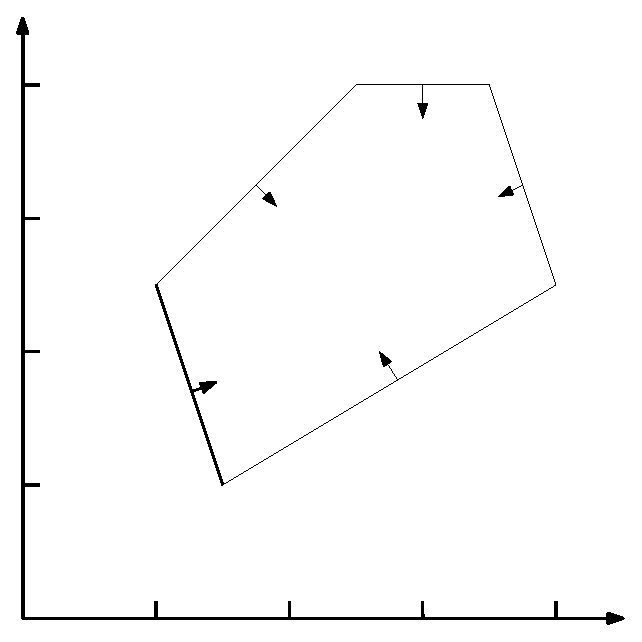
\includegraphics[width=6cm]{cutting_plane005.eps} 
            \end{center}
        \end{minipage}        
\end{frame}

\begin{frame}[t]{The Cutting Plane Method (3)}
        \begin{minipage}[t]{0.48\textwidth}
            LP solution:
            \begin{itemize}
                \item $ x_2 \geq -3x_1 + 5.5 $
                \item $ x_2 \leq x_1 + 1.5 $
                \item $ x_2 \leq 4$
                \item $ x_2 \leq -3x_1 + 14.5 $
                \item $ x_2 \geq 0.6x+1 + 0.1 $
                \item \alert{$ \max 4x_1 + x_2 $}
            \end{itemize}
        \end{minipage}
        \begin{minipage}[t]{0.48\textwidth}
            \begin{center}
                \includegraphics[width=6cm]{cutting_plane006.eps} 
            \end{center}
        \end{minipage}        
\end{frame}

\begin{frame}[t]{The Cutting Plane Method (3)}
        \begin{minipage}[t]{0.48\textwidth}
            ILP solution:
            \begin{itemize}
                \item \alert{$ \max 4x_1 + x_2 $}
            \end{itemize}
        \end{minipage}
        \begin{minipage}[t]{0.48\textwidth}
            \begin{center}
                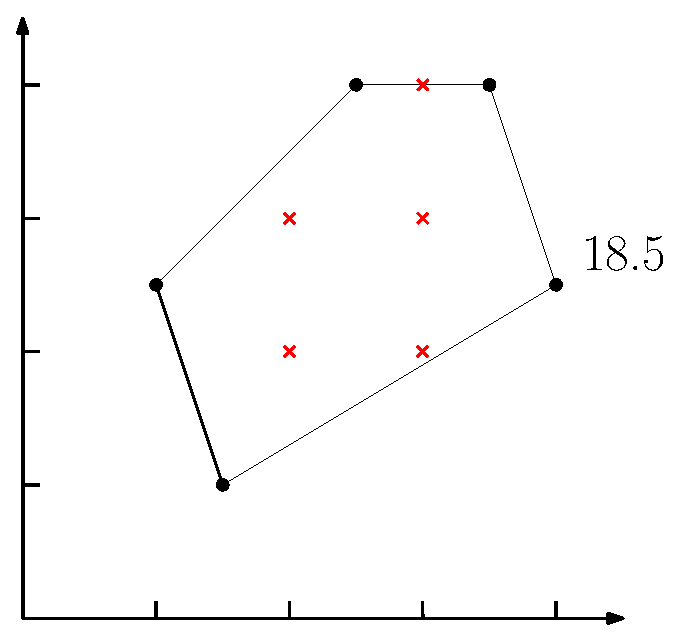
\includegraphics[width=6cm]{cutting_plane007.eps} 
            \end{center}
        \end{minipage}        
\end{frame}

\begin{frame}[t]{The Cutting Plane Method (3)}
        \begin{minipage}[t]{0.48\textwidth}
            ILP solution:
            \begin{itemize}
                \item \alert{$ \max 4x_1 + x_2 $}
                \item Integrality gap
            \end{itemize}
        \end{minipage}
        \begin{minipage}[t]{0.48\textwidth}
            \begin{center}
                \includegraphics[width=6cm]{cutting_plane008.eps} 
            \end{center}
        \end{minipage}        
\end{frame}

\begin{frame}[t]{The Cutting Plane Method (3)}
        \begin{minipage}[t]{0.48\textwidth}
            ILP solution:
            \begin{itemize}
                \item \alert{$ \max 4x_1 + x_2 $}
                \item Integrality gap
                \item Convex hull of integer points
            \end{itemize}
        \end{minipage}
        \begin{minipage}[t]{0.48\textwidth}
            \begin{center}
                \includegraphics[width=6cm]{cutting_plane009.eps} 
            \end{center}
        \end{minipage}        
\end{frame}

\begin{frame}[t]{The Cutting Plane Method (3)}
        \begin{minipage}[t]{0.48\textwidth}
            ILP solution:
            \begin{itemize}
                \item \alert{$ \max 4x_1 + x_2 $}
                \item Integrality gap
                \item Convex hull of integer points
                \item Valid inequalities
            \end{itemize}
        \end{minipage}
        \begin{minipage}[t]{0.48\textwidth}
            \begin{center}
                \includegraphics[width=6cm]{cutting_plane010.eps} 
            \end{center}
        \end{minipage}        
\end{frame}

\begin{frame}[t]{The Cutting Plane Method (3)}
        \begin{minipage}[t]{0.48\textwidth}
            ILP solution:
            \begin{itemize}
                \item \alert{$ \max 4x_1 + x_2 $}
                \item Integrality gap
                \item Convex hull of integer points
                \item Valid inequalities
            \end{itemize}
        \end{minipage}
        \begin{minipage}[t]{0.48\textwidth}
            \begin{center}
                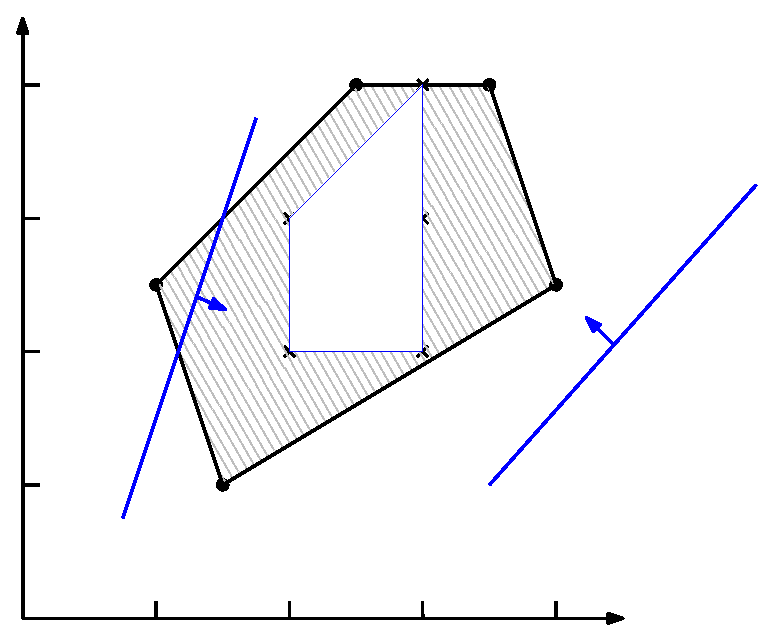
\includegraphics[width=6cm]{cutting_plane011.eps} 
            \end{center}
        \end{minipage}        
\end{frame}

\begin{frame}[t]{The Cutting Plane Method (3)}
        \begin{minipage}[t]{0.48\textwidth}
            ILP solution:
            \begin{itemize}
                \item \alert{$ \max 4x_1 + x_2 $}
                \item Integrality gap
                \item Convex hull of integer points
                \item Valid inequalities
            \end{itemize}
        \end{minipage}
        \begin{minipage}[t]{0.48\textwidth}
            \begin{center}
                \includegraphics[width=6cm]{cutting_plane012.eps} 
            \end{center}
        \end{minipage}        
\end{frame}

\begin{frame}[t]{The Cutting Plane Method (3)}
        \begin{minipage}[t]{0.48\textwidth}
            ILP solution:
            \begin{itemize}
                \item \alert{$ \max 4x_1 + x_2 $}
                \item Integrality gap
                \item Convex hull of integer points
                \item Valid inequalities
            \end{itemize}
        \end{minipage}
        \begin{minipage}[t]{0.48\textwidth}
            \begin{center}
                \includegraphics[width=6cm]{cutting_plane013.eps} 
            \end{center}
        \end{minipage}        
\end{frame}


\begin{frame}[t]{The Branch-and-Bound Method (1)}
    \begin{itemize}
        \item<1-> Certain method for finding the optimal to an ILP
        \item<2-> Searches the entire solution space
        \item<3-> [ ]
            \begin{align}
                \text {max }  \mathbf{c} \cdot \mathbf{x}   \nonumber\\
                \mathbf{A} \mathbf{x}   \leq \mathbf{b}     \nonumber\\
                \mathbf{x} \in \{ 0, \, 1 \}^{n}            \nonumber
            \end{align}
         \item<4-> LP relaxation: 
            \begin{align}
                \text {max }  \mathbf{c} \cdot \mathbf{x}   \nonumber\\
                \mathbf{A} \mathbf{x}   \leq \mathbf{b}     \nonumber\\
                \mathbf{x} \in [ 0, \, 1 ]^{n}            \nonumber
            \end{align}
    \end{itemize}
\end{frame}

\begin{frame}[t]{The Branch-and-Bound Method (2)}
    Solving the LP relaxation
    \begin{center}
        \includegraphics[width=10cm]{b_and_b000.eps} 
    \end{center}
\end{frame}

\begin{frame}[t]{The Branch-and-Bound Method (2)}
    Fixing variables
    \begin{center}
        \includegraphics[width=10cm]{b_and_b001.eps} 
    \end{center}
\end{frame}

\begin{frame}[t]{The Branch-and-Bound Method (2)}
    Fixing variables
    \begin{center}
        \includegraphics[width=10cm]{b_and_b002.eps} 
    \end{center}
\end{frame}

\begin{frame}[t]{The Branch-and-Bound Method (2)}
    Fixing variables
    \begin{center}
        \includegraphics[width=10cm]{b_and_b003.eps} 
    \end{center}
\end{frame}

\begin{frame}[t]{The Branch-and-Bound Method (2)}
    The bounding phase (pruning)
    \begin{center}
        \includegraphics[width=10cm]{b_and_b004.eps} 
    \end{center}
\end{frame}

\begin{frame}[t]{The Branch-and-Bound Method (2)}
    The bounding phase (pruning)
    \begin{center}
        \includegraphics[width=10cm]{b_and_b005.eps} 
    \end{center}
\end{frame}

\begin{frame}[t]{The Branch-and-Bound Method (2)}
    How to get good lower bounds?
    \begin{center}
        \includegraphics[width=10cm]{b_and_b006.eps} 
    \end{center}
\end{frame}

\begin{frame}[t]{The Branch-and-Bound Method (2)}
    How to get good lower bounds?
    \begin{center}
        \includegraphics[width=10cm]{b_and_b007.eps} 
    \end{center}
\end{frame}


%%%%%%%%%%%%%%%%%%%%%%%%%%%%%%%%%%%%%%%%%%%%%%%%%%%%%%%%%%%%%%%%%%%%%%%%%%%%%%%%%%%%%%%%%%%%%%%%%%%%%%%%%%%%%%%%%%%%%%%%%%%%%%%
\section{A Branch-and-Cut Algorithm for PCTSP}

\begin{frame}[t]{PCTSP Recap}
\begin{itemize}
\item An instance of the Prize Collecting TSP:
\begin{figure}
	\centering
	\begin{tikzpicture}
        
        \draw (0, 0) node[circle, inner sep=1pt, fill=black, label={below:{$depot$}}] (D) {}; 
        \draw (1, 1) node[circle, inner sep=1pt, fill=black] (A) {}; 
        \draw (3, 2) node[circle, inner sep=1pt, fill=black] (B) {}; 
        \draw (-3, 3) node[circle, inner sep=1pt, fill=black] (C) {}; 
        \draw (-1, 4) node[circle, inner sep=1pt, fill=black] (E) {}; 
        \draw (0, 3) node[circle, inner sep=1pt, fill=black] (F) {}; 
        \draw (2, 3) node[circle, inner sep=1pt, fill=black] (G) {}; 
         \draw (-3, 1) node[circle, inner sep=1pt, fill=black, label={below:{$v$}}] (v) {}; 
        \draw (-2, 2) node[circle, inner sep=1pt, fill=black, label={below:{$u$}}] (u) {};         
        \node at (-2.5, 1.5) (m) {};
        \node at (-4, 1.5) (n) {$c_{uv}$};
        
        \draw [->, color = red] (m) to [bend right = 45] (n);
        \draw [fill = blue, dashed, thick] (u) to (v);

    	\node[above = 0.2cm] at (-2, 2) {$\beta_u$};
	\end{tikzpicture}
\end{figure}
\end{itemize}
\end{frame}

\begin{frame}[t]{ILP Formulation (1)}
    \begin{itemize}
        \item<1-> Two sets of decision variables:
        \item<2-> For every vertex $i \in S$:
        \[
            y_j =
                \begin{cases}
                    1 & \text{if vertex $j$ is selected in the optimal tour} \\
                    0 & \text{otherwise}
                \end{cases}
        \]       
        \item<3-> For every edge $e \in E$:
        \[
            x_e =
                \begin{cases}
                    1 & \text{if edge $e$ is selected in the optimal tour} \\
                    0 & \text{otherwise}
                \end{cases}
        \]        
    \end{itemize}
\end{frame}

\begin{frame}[t]{ILP Formulation (2)}
    \begin{align} 
        \text {max } \label{pctsp_obj}     & \sum_{j\in S} \beta_j y_j  -     \sum_{e\in E} c_e x_e &
        \\
        \text{subject to } \nonumber    &  & \\
        \label{const:pctsp1}               & \sum_{e \in \delta(i)} x_e = 2 y_{i}  & \forall i \in S \\
        \label{const:pctsp2}               & \sum_{e \in E(V) } x_e \leq \sum_{i \in V \backslash\{ k \}} y_{i} & \forall k \in V, V\subseteq S' \\
        \label{const:pctsp3}               & y_r = 1 \\
        \label{const:pctsp4}               & x_e \in \{0, \, 1\}, \, y_j \in \{0, \, 1\}  
    \end{align}
\end{frame}

\begin{frame}[t]{ILP Formulation (3)}
    \begin{itemize}
        \item<1-> Generalized Subtour Elimination Constraints (GSECs) for PCTSP:
        \[  \sum_{e \in E(V) } x_e \leq \sum_{i \in V \backslash\{ k \}} y_{i} \qquad \forall k \in V, V\subseteq S' \] 
        \item<2-> Subtour Elimination Constraints for TSP:
        \[  \sum_{e \in E(V) } x_e \leq \abs{V} - 1 \qquad \forall V \subseteq S' \]         
        \item<2-> Problem: there are exponentially many GSECs
        \item<3-> Solution: do not introduce them all at once (cutting plane method)
            \begin{itemize}
                \item<5-> Start with an initial set of constraints and solve the LP relaxation
                \item<6-> Identify violated constraints (if any) and add them to the model (\textbf{Separation} problem)
                \item<7-> Resolve and iterate until completion
            \end{itemize}    
    \end{itemize}
\end{frame}


\begin{frame}{A Branch-and-Cut Algorithm for PCTSP}
\begin{center}
        \includegraphics[width=7cm]{Branch_and_Cut.eps} 
\end{center}
\end{frame}

\begin{frame}[t]{In This Research}
    \begin{itemize}
        \item<1-> We developed a \alert{Branch-and-Cut} algorithm to find exact solutions of PCTSP
            \begin{itemize}
                \item<2-> Strengthen the LP relaxation by two sets of valid inequaities:
                    \begin{enumerate}
                        \item<3-> GSECs
                        \item<4-> Primitive Comb Inequalities
                    \end{enumerate}
                \item<5-> Adapted \textbf{separation heuristics} for GSECs and Primitive Combs from similar heuristics for TSP
                \item<6-> Used a  local search heuristic to \textbf{round} fractional solutions
                \item<7-> Developed and adapted \textbf{branching heuristics}
            \end{itemize}
    \end{itemize}
\end{frame}

\begin{frame}[t]{Computational Results}
    \begin{table}
        \begin{center}
            \resizebox{.75\textwidth}{!}
            {
                \begin{tabular}{l l l l l l l}
                    \hline \\
                    \textbf{Instance}	&	\textbf{Obj.}	&	\textbf{ILP Time}	&	\textbf{Optimal}	&	\textbf{Time}	&	\textbf{\% Gap}	& \\
                    \hline \\
                    att48		&	-1358.75	&	1		&	\checkmark	&	<1		&			&	\\
                    st70		&	6432.24	    &	3		&	\checkmark	&	4		&			&	\\
                    eilD76		&	6774.3		&	2		&	\checkmark	&	8		&			&	\\
                    gr96		&	9527.97	    &	6		&	\checkmark	&	46		&			&	\\
                    ch150		&	8827.78	    &	14226	&	\checkmark	&	1166	&			&	\\
                    kroB200		&	3151.54	    &	t.l.	&	\checkmark	&	270		&			&	\\
                    a280		&	24878.5	    &	t.l.	&	\checkmark	&	3550	&			&	\\
                    fl417		&   <41424	    &	t.l.	&	-			&	t.l.	&	\%0.05	&	\\
                    gr431		&	41742.6	    &	5180	&	\checkmark	&	2651	&			&	\\
                    pr439		&	384.1	    &	t.l.	&	\checkmark	&	1502	&			&	\\
                    pcb442		&   <43514.9    &	t.l.	&	-			&	t.l.	&	\%0.07	&	\\
                    d493		&   <48946.8	&	t.l.	&	-			&	t.l.	&	\%0.02	&	\\
                    p654		&	<65493		&	t.l.	&	-			&	t.l.	&	\%0.02	&	\\
                    d657		&	<64690.2	&	t.l.	&	-			&	t.l.	&	\%0.03	&	\\
                    \hline
                \end{tabular} }
            \caption{Computational results for the \textbf{Smart Branch}} \label{tbl:results3}
        \end{center}
    \end{table}
\end{frame}

\begin{frame}[t]{Papers and Presentations}
    \begin{itemize}
        \item B. Chan, E. Iranmanesh, K. K., R. Krishnamurti, A. Rafiey, V. Sokol: \textbf{A Column Generation Approach for the Vehicle Routing Problem with Skill Sets}, \emph{CORS 2013}
        \item K. K., R. Krishnamurti: \textbf{Prize Collecting Travelling Salesman Problem - Fast Heuristic Separations}, \emph{ICORES 2016}
    \end{itemize}
\end{frame}

\plain{Thank You!}

\begin{frame}{Questions}
    \begin{center}
        \includegraphics[width=7cm]{qmark.jpeg}
    \end{center}
\end{frame}

\begin{frame}[t]{The Algorithm}
    \begin{enumerate}
        \item<1-> Initialize the list of problems $L$ to \textsc{NULL}
        \item<2-> Add the first LP relaxation to $L$
        \item<3-> Pop the front of $L$ to get the problem $P$
        \item<4-> Solve $P$ to get $z^*$
        \item<5-> Round the fractional solution to get a lower bound
        \item<6-> If the best lower bound is larger than $z^*$, go to 3
        \item<7-> If there are violated constraints, add \emph{some} cuts to $P$
        \item<8-> If the solution is not feasible, go to 4
        \item<9-> If the solution is integral, update the best lower bound and go to 3
        \item<9-> Fix a variable and get $P_0$ and $P_1$
        \item<10-> Add $P_0$ and $P_1$ to the \alert{front} of $L$
        \item<11-> If $L$ is not empty, then go to 3
        \item<12-> Report the best lower bound
    \end{enumerate}
\end{frame}

\begin{frame}[fragile]{Exact Separation of GSECs}
\begin{itemize}
    \item<1-> Solve a linear relaxation of the PCTSP formulation
    \item<2-> Get the solution $(x^*, \, y^*)$ 
    \item<3-> For every node $k \in S'$:
    \begin{align} 
        \zeta_k \ \text  = \ {max } \label{sep_obj} & \sum_{e\in E'} x_e^{*} w_e  - \sum_{j \in S' \backslash \{ k \}}  y_j^{*} z_j     &  \\
        \text{subject to }                          & & \nonumber \\
        \label{const:sep1}                          & w_e\leq z_i, w_e\leq z_j  & \forall e =(i,j) \in E' \\
        \label{const:sep2}                          & w_e \geq z_i + z_j - 1    & \forall e = (i,j) \in E' \\
        \label{const:sep3}                          & w_e \in \{0,1\}, z_j \in \{0,1\}, z_k = 1   & \forall e \in E', \forall j \in S'
    \end{align}
    \item<4-> A strictly positive $\zeta_k$ means a violated GSEC
    \item<5-> Solvable in polynomial time but \alert{time consuming!}
\end{itemize}
\end{frame}

\begin{frame}{Heuristic Separation}
\begin{itemize}
\item<1-> Equivalent cut-set representation of GSECs:
\begin{align}
\label{eq:cut-set}
& \sum_{ e \in E(V, \, S' \, \backslash \, V) } x_{e} - 2 y_{k} \geq 0   \hspace {2cm}   \forall k \in V, V \subseteq S'
\end{align}
(due to degree constraints and GSECs)
\item<2-> Can be transformed to a flow problem 
\item<3->  Find the cut that minimizes:
\begin{align}
\label{eq:min-cut}
\sum_{ e \in E(V, \, S' \, \backslash \, V) } x_{e} - 2 \max_{k \in V} \{ y_{k} \}.
\end{align}
\item<4-> We have adapted a shrinking heuristic from TSP which can help us identify the nodes that will end up on the same side of the \alert{shore} for the cut $(V, \, S' \, \backslash \, V)$
\end{itemize}
\end{frame}

\end{document}
